\section{Motivation and Background}
\label{background}

GPU performance has scaled well over the last 10 years fueled by a significant 
growth in per-GPU transistor count.  For example, in 2010 Nvidia's Fermi 
generation GPUs contained 1.95B transistors with a die size of 
529mm\textsuperscript{2} and as of 2016, Nvidia's Pascal generation contains 
12B transistors and is 610 mm\textsuperscript{2}. As transistor density growth 
slows, GPU manufacturers have to look beyond node scaling to alternative 
solutions for increasing transistor count and performance. While GPU die sizes 
have been increasing quickly over the past several generations, this growth is 
expected to slow down due to limitations in lithography and manufacturing 
costs. 

Without larger or denser dies, GPU manufacturers will need to turn to 
alternative technologies to increase transistor count.  One possibility is 
moving to 3D die-stacking as a solution for continued transistor growth. 
Unfortunately 3D die-stacking still has a significant number of engineering 
challenges related to power delivery, energy density, and 
cooling~\cite{verbree2010cost} when employed in maximal die-sized chips such as 
GPUs and moving beyond a 2 high stack to 4 or 8 stacks will be even more 
difficult. Because of these challenges, GPU manufacturers are likely to 
consider a tried and trued solution in the CPU world to gain additional 
transistor count, 
\textit{multi-socket GPUs}.

\begin{figure*}[tp]
    \centering
    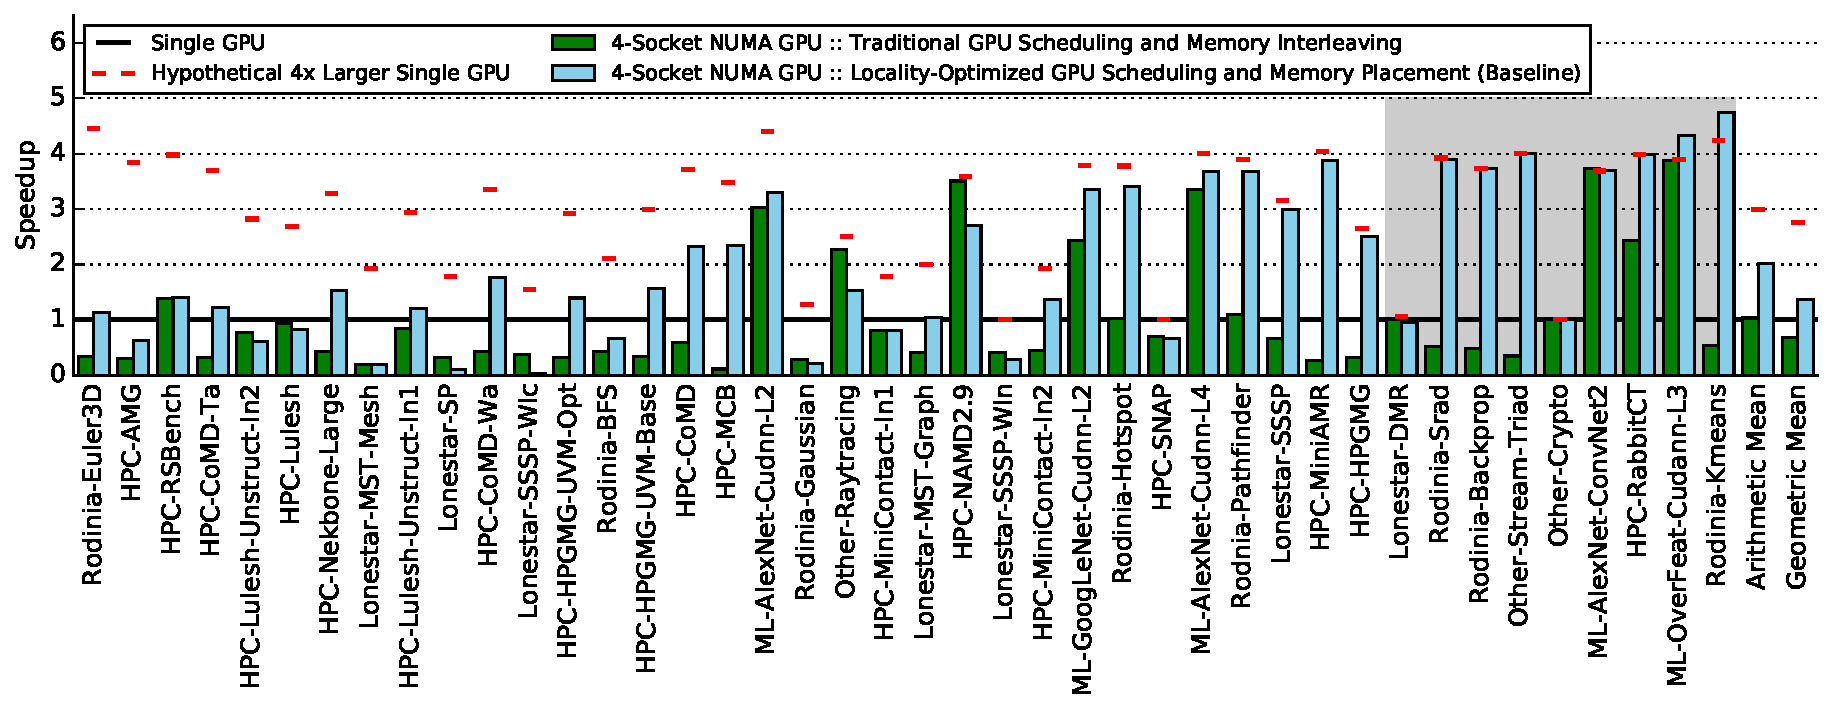
\includegraphics[width=1.0\linewidth]{figures/plot_different_baselines.pdf}
    \caption{Relative performance of a 4-socket NUMA GPU using to a single GPU 
and a hypothetical 4$\times$ larger (all resources scaled) single GPU showing 
upper bound of performance this application can achieve via GPU hardware 
scaling. Applications shown in grey achieve XXX\% of theoretical scaling without 
microarchitectural modification.}
    \label{fig:motivation}
\end{figure*}

The evolution of GPU computing has moved from PCIe attached peripherals to full 
systems designed around the GPU as the primary computing engine.  These systems 
have custom PCB layouts that accomodate multiple high pin count socketed 
GPUs~\cite{DGX} that have GPU to GPU interconnects that resemble QPI or 
Hypertransport~\cite{INTELQPI,AMDHT} much more than legacy PCIe interfaces.  
Despite the improvement in hardware capabilities, to-date these multi-GPU 
solutions have been exposed as single GPU solutions with improved GPU--GPU 
interconnects.  While multi-GPU systems can provide high aggregate throughput, 
the programming model for multi-GPU systems has diverged from the single GPU 
programming model and requires layering additional software runtimes like MPI 
or openshmem on top of the native GPU programming model (CUDA or openCL).  By 
requiring re-writing of the GPU application to enable multi-GPU performance, 
many applications never are ported to use multiple GPUs.

In this work, we examine the performance achievable by architecting a 
multi-socket NUMA-aware single GPU.  Building upon existing work in the 
NUMA-CPU and GPU community, we first describe the basic multi-socket GPU runtime 
that allows a multi-socket GPU system to be exposed to GPU developers as a 
single GPU and exploits some well known scheduling and memory locality 
optimizations for NUMA systems. We then look at the performance implications 
that this multi-socket NUMA design has on applications that have been optimized 
for a traditional single GPU.  We identify that current GPU interconnect 
utilization and cache policies are sub-optimal for a multi-socket NUMA GPU and 
show how these problems can largely be overcome with architectural innovation.  
Finally, we examine the scaling efficiency of a multi-socket NUMA-aware GPU to 
understand if NUMA-aware GPUs will see significantly improve performance  
without any code-rewriting required by the application programmer.
\\\\
\textbf{A Multi-Socket GPU Runtime}
\\\\
\noindent As demonstrated by Cabezas et al.~\cite{Cabezas2015} it is possible to design 
a framework and a runtime system that transparently decomposes GPU kernels in 
sub-kernels and executes them on multiple GPUs in parallel. On the Nvidia 
GPUs, this is doable by intercepting and remapping each single kernel call, 
GPU memory allocation, GPU memory copy and GPU wide synchronization issued by 
the CUDA driver. Special care needs to be put (i) to the GPU local memory 
fences which needs to be promoted to system level and (ii) to the 
sub-kernels CTA identifiers which needs to be properly corrected to 
reflect those in the original kernel call. 
 
In ~\cite{Cabezas2015} these two problems were solved by introducing  
code annotations and an additional source-to-source compiler which was also 
responsible for statically assigning data and computation on each GPU. In our 
work, we follow a very similar strategy but we do not use any additional 
compiler for two reasons (i) we use a simulated environment in which 
we can properly model the requirements for system wide memory fences 
and sub-kernel to kernel CTA identifiers mapping (ii) we model a system 
which implements UVM page migration of on demand as recently introduced in the 
Tesla P100 GPU~\cite{P100}. UVM page migration allows to allocate 
all the memory upfront in system memory and to transparently migrate pages 
on the GPU memory on demand as soon as the first access (also called first 
touch) 
is performed.

For sake of completion, while on a single GPU the interleaving of memory at 
the granularity of single cache line is routinely done to reduce memory 
camping effects and to maximize bandwidth, doing it across multiple GPUs 
disrupts locality and it can result in large amount of remote accesses even 
for regular and dense applications. In the same way, while on a single GPU 
fine grain dynamic assignment of CTAs to the SMs is performed to achieve good 
load balancing, extending it on a Multi-GPU system (for instance creating a 
large amount of small sub-kernels) results in huge overhead due to the cost 
of starting a single sub-kernel.

For this reason as done in~\cite{Cabezas2015}, we decompose a single kernel 
in only N sub-kernels, where N is the total number of GPUs in the system, and 
we assign to each GPU an equal amount of CTAs. We also select CTAs in each 
sub-kernel to be contiguous even if it could expose workload unbalance across 
CTAs, still to preserve locality present in many dense and regular applications 
where contiguous CTAs access contiguous memory. 

In general the problems of data placement and task placement (minimizing 
remote data access and ensuring load balancing) can not be completely 
decoupled and pathological case can always be found.
However across our benchmark suites, we found first touch page placement and 
contiguous CTA block scheduling to be the most reasonable choice, 
again because it preserves locality when present. We will therefore use this 
as the baseline architecture for our studies in the rest of this paper.

In Figure~\ref{fig:motivation} we show the relative performance of our 
baseline NUMA multi-socket 4 GPUs system connected with a switch in which the 
link bandwidth is 64 GB/sec (comparable to NVlink) with respect to a single 
GPU (composed of 64 SMs with 768 GB/sec of memory bandwidth). A more detailed 
description of the methodology and simulation parameters is in 
Section~\ref{methodology}. Also in Figure we show with a red dash the 
performance achievable by an Hypothetical UMA multi-socket 4 GPUs, in which 
the interconnect bandwidth matches the memory bandwidth. This red mark 
represent a good approximation of the maximum theoretical performance we 
could expect from our NUMA system. We sorted the applications by the gap 
between relative performance of the baseline and maximum theoretical 
performance. We can see that on the right side part of the graph some 
applications (that are not sensitive to interconnect bandwidth) already 
achieve the maximum theoretical performance, while on the left there is quite 
large gap. In the rest of this paper we present techniques aimed to reduce 
this gap. To simplify the discussion we will exclude the benchmarks that 
already achieve 99\% of the theoretical performance when explaining these 
techniques. We will re-include them in the final plots to demonstrate that 
there was not performance regression. 